\documentclass{article}

\usepackage[T1]{fontenc}    %Schriftart des Dokumentes
\usepackage[ngerman]{babel} %Dokumentensprache, hier Deutsch
\usepackage{amsmath, amssymb, stmaryrd} %mathematische Schriftzeichen
\usepackage{graphicx} %Einfügen von Grafiken
\usepackage{wrapfig}
\usepackage{bm}
\usepackage{subfig}
\usepackage{newclude}
\usepackage{pdfpages}
\usepackage{hyperref}
\hypersetup{
    colorlinks,
    citecolor=black,
    filecolor=black,
    linkcolor=black,
    urlcolor=black
}

\makeatletter
\newcommand\invisiblesection[1]{%
  \refstepcounter{section}%
  \addcontentsline{toc}{section}{\protect\numberline{\thesection}#1}%
  \sectionmark{#1}\phantom{}}
\makeatother

\setlength{\parindent}{0pt} %Einrückung von Absätzen auf null gesetzt
\setlength{\parskip}{10pt} %Abstand zischen Absätzen auf 10pt gesetzt

\title{Versuch 243: Bestimmung der Boltzmannkonstante mit Hilfe von thermischem Rauschen}
\author{Matthias Kuntz}
\date{03.06.2024}

\renewcommand*\contentsname{Zusammenfassung}

\begin{document}

\maketitle

\tableofcontents

\newpage

%-------------------------EINLEITUNG-------------------------
\section{Einleitung}

Als Weiterführung des ersten Versuchs zur Bestimmung der Boltzmannkonstante soll dieser einen alternativen Weg beschreiben, wie man mithilfe Brownscher Bewegung die Boltzmannkonstante bestimmen kann.


\subsection{Physikalische Grundlagen}

Als thermisches Rauschen bezeichnet man die Brownsche Bewegung von Ladungsträgern in einem elektrischen Leiter bei Temperaturen über 0K. Selbst ohne anliegende Spannung entstehen so statistisch variierende elektrische Potenziale im Leiter, welche mit einem sehr empfindlichen Oszilloskop messbar sind. Diese sogenannte Rauschspannung $U_r$ lässt sich ohne anliegende äußere Spannung folgendermaßen beschreiben:

\begin{equation}
    \langle U_r \rangle = \lim_{t' \rightarrow \infty} \frac{1}{t'} \int_{0}^{t'} U_r(t) dt = 0
\end{equation}

Wie bei jeder Brownschen Bewegung verschwindet der Mittelwert aufgrund der ungerichteten zufälligen Bewegung. Zur Quantifizieren benötigen wir den Effektivwert der Spannung:

\begin{equation}
    \sqrt{\langle U_r^2 \rangle} = \sqrt{\lim_{t' \rightarrow \infty} \frac{1}{t'} \int_{0}^{t'} U_r^2(t) dt}.
\end{equation}

Untersucht man das Frequenzspektrum der entstehenden Rauschspannung, so stellt man fest, dass alle Frequenzen gleich häufig vorkommen, weshalb es auch als weißes Rauschen bezeichnet wird. 

Wichtig ist die Nyquist-Beziehung für den quadratischen Effektivwert

\begin{equation}
    \langle U_r^2 \rangle = 4 k_B T R \ \Delta f,
\end{equation}

welche diesen in Abhängigkeit der Boltzmannkonstante $k_B$, der Temperatur $T$, dem ohmschen Widerstand $R$ und der Bandbreite $\Delta f$ angibt und uns in diesem Versuch die Bestimmung der Boltzmannkonstante ermöglicht.

Da die Rauschspannung bei Raumtemperatur bei einem realen Widerstand enorm gering ist, benötigen wir zusätzlich einen Verstärker, der diese um das 1000-fache verstärkt, sodass diese problemlos messbar wird. Hierbei ist allerdings der Verstärker selbst als Rauschquelle zu beachten. Unsere gemessene Rauschspannung wird sich also aus der des Widerstands und der des Verstärkers zusammensetzen:

\begin{equation}
    \langle U_{r+v}^2 \rangle = \langle U_r^2 \rangle + \langle U_v^2 \rangle
\end{equation}

Das Verstärkerrauschen muss also zunächst separat bestimmt und im Anschluss von der Hauptmessung abgezogen werden. 

Des Weiteren wird in diesem Versuch ein zusätzlicher Bandpassfilter verwendet, welche die Kanten der Bandbreite verschärft und somit den ungenauen flacheren Abfall des Widerstands verbessert. 

Zur genauen Bestimmung der Boltzmannkonstante betrachten wir den Frequenzgang $g(f)$ der Messelektronik:

\begin{equation}
    g(f) = \frac{U_{aus}}{U_{ein}} \bigg|_f .
\end{equation}

Hierbei entspricht $U_{ein}$ der Rauschspannung $U_r$ und $U_{aus}$ der gemessenen Ausgangsspannung des Bandpassfilters, weshalb wir mit der Nyquist-Beziehung und der Substitution

\begin{equation}
    B = \int_{0}^{\infty} g(f)^2 df
\end{equation}

die folgende Formel für die Boltzmannkonstante erhalten:

\begin{equation}
    k_B = \frac{\langle U_{aus}^2 \rangle - \langle U_{v}^2 \rangle}{4 T R B}.
    \label{eq:Boltzmann}
\end{equation}

Hierbei ist $B$ numerisch aus dem gemessenen $g(f)$ zu berechnen.

Zur Messung des Frequenzgangs dient ein Funktionsgenerator, welcher um das 1000-fache abgeschwächt wird, damit der Verstärker nicht in Sättigung geht. Wir haben also eine Dämpfung $D=10^{-3}$. Somit folgt bei uns für den Frequenzgang:

\begin{equation}
    g(f)= \frac{1}{D} \frac{\sqrt{\langle U_{aus}^2 \rangle}}{\sqrt{\langle U_{ein}^2 \rangle}}.
    \label{eq:Frequenzgang}
\end{equation}

\newpage
\subsection{Versuchsaufbau}

Der Aufbau, dargestellt in Abbildung \ref{fig:Aufbau}, besteht im Grunde aus den bereits genannte Bauteilen: einem einstellbaren ohmschen Widerstand als elektrischer Leiter zur Entstehung von Rauschspannung, einem Verstärker und Bandpassfilter, einem Dämpfungsglied für den Signalgenerator bei der Frequenzgangmessung, jenem Signalgenerator und einem Effektivwert-Voltmeter. Letzteres sendet dabei die Signale direkt an einen Computer, wo diese digital abgespeichert werden. 

\phantom{.}

\begin{figure}[!h]
    \centering
    \resizebox{0.9\textwidth}{!}{
    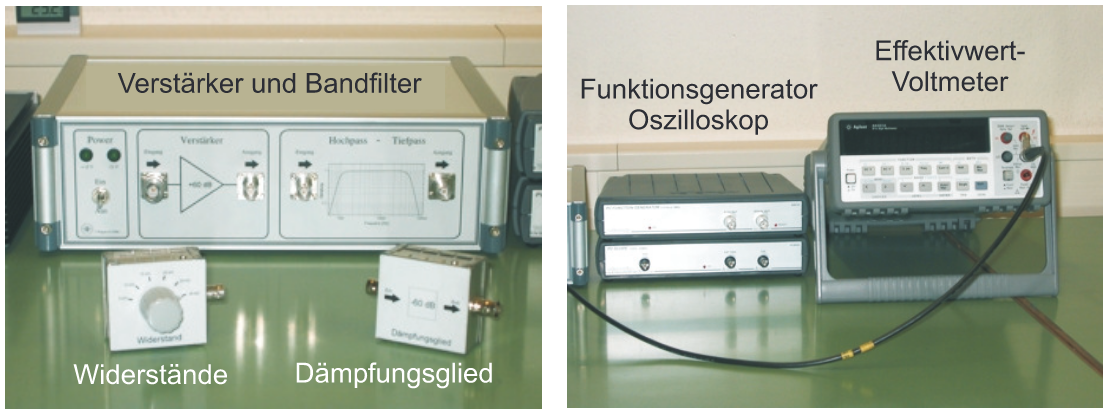
\includegraphics{graphics/aufbau.png}}
    \caption{Versuchsaufbau [Quelle: PAP2.2 Skript, S.33, Stand: 25.06.2024]}
    \label{fig:Aufbau}
\end{figure}





%---------------VERSUCHSPROTOKOLL MIT MESSDATEN---------------
\newpage

\section{Versuchsprotokoll mit Messdaten}

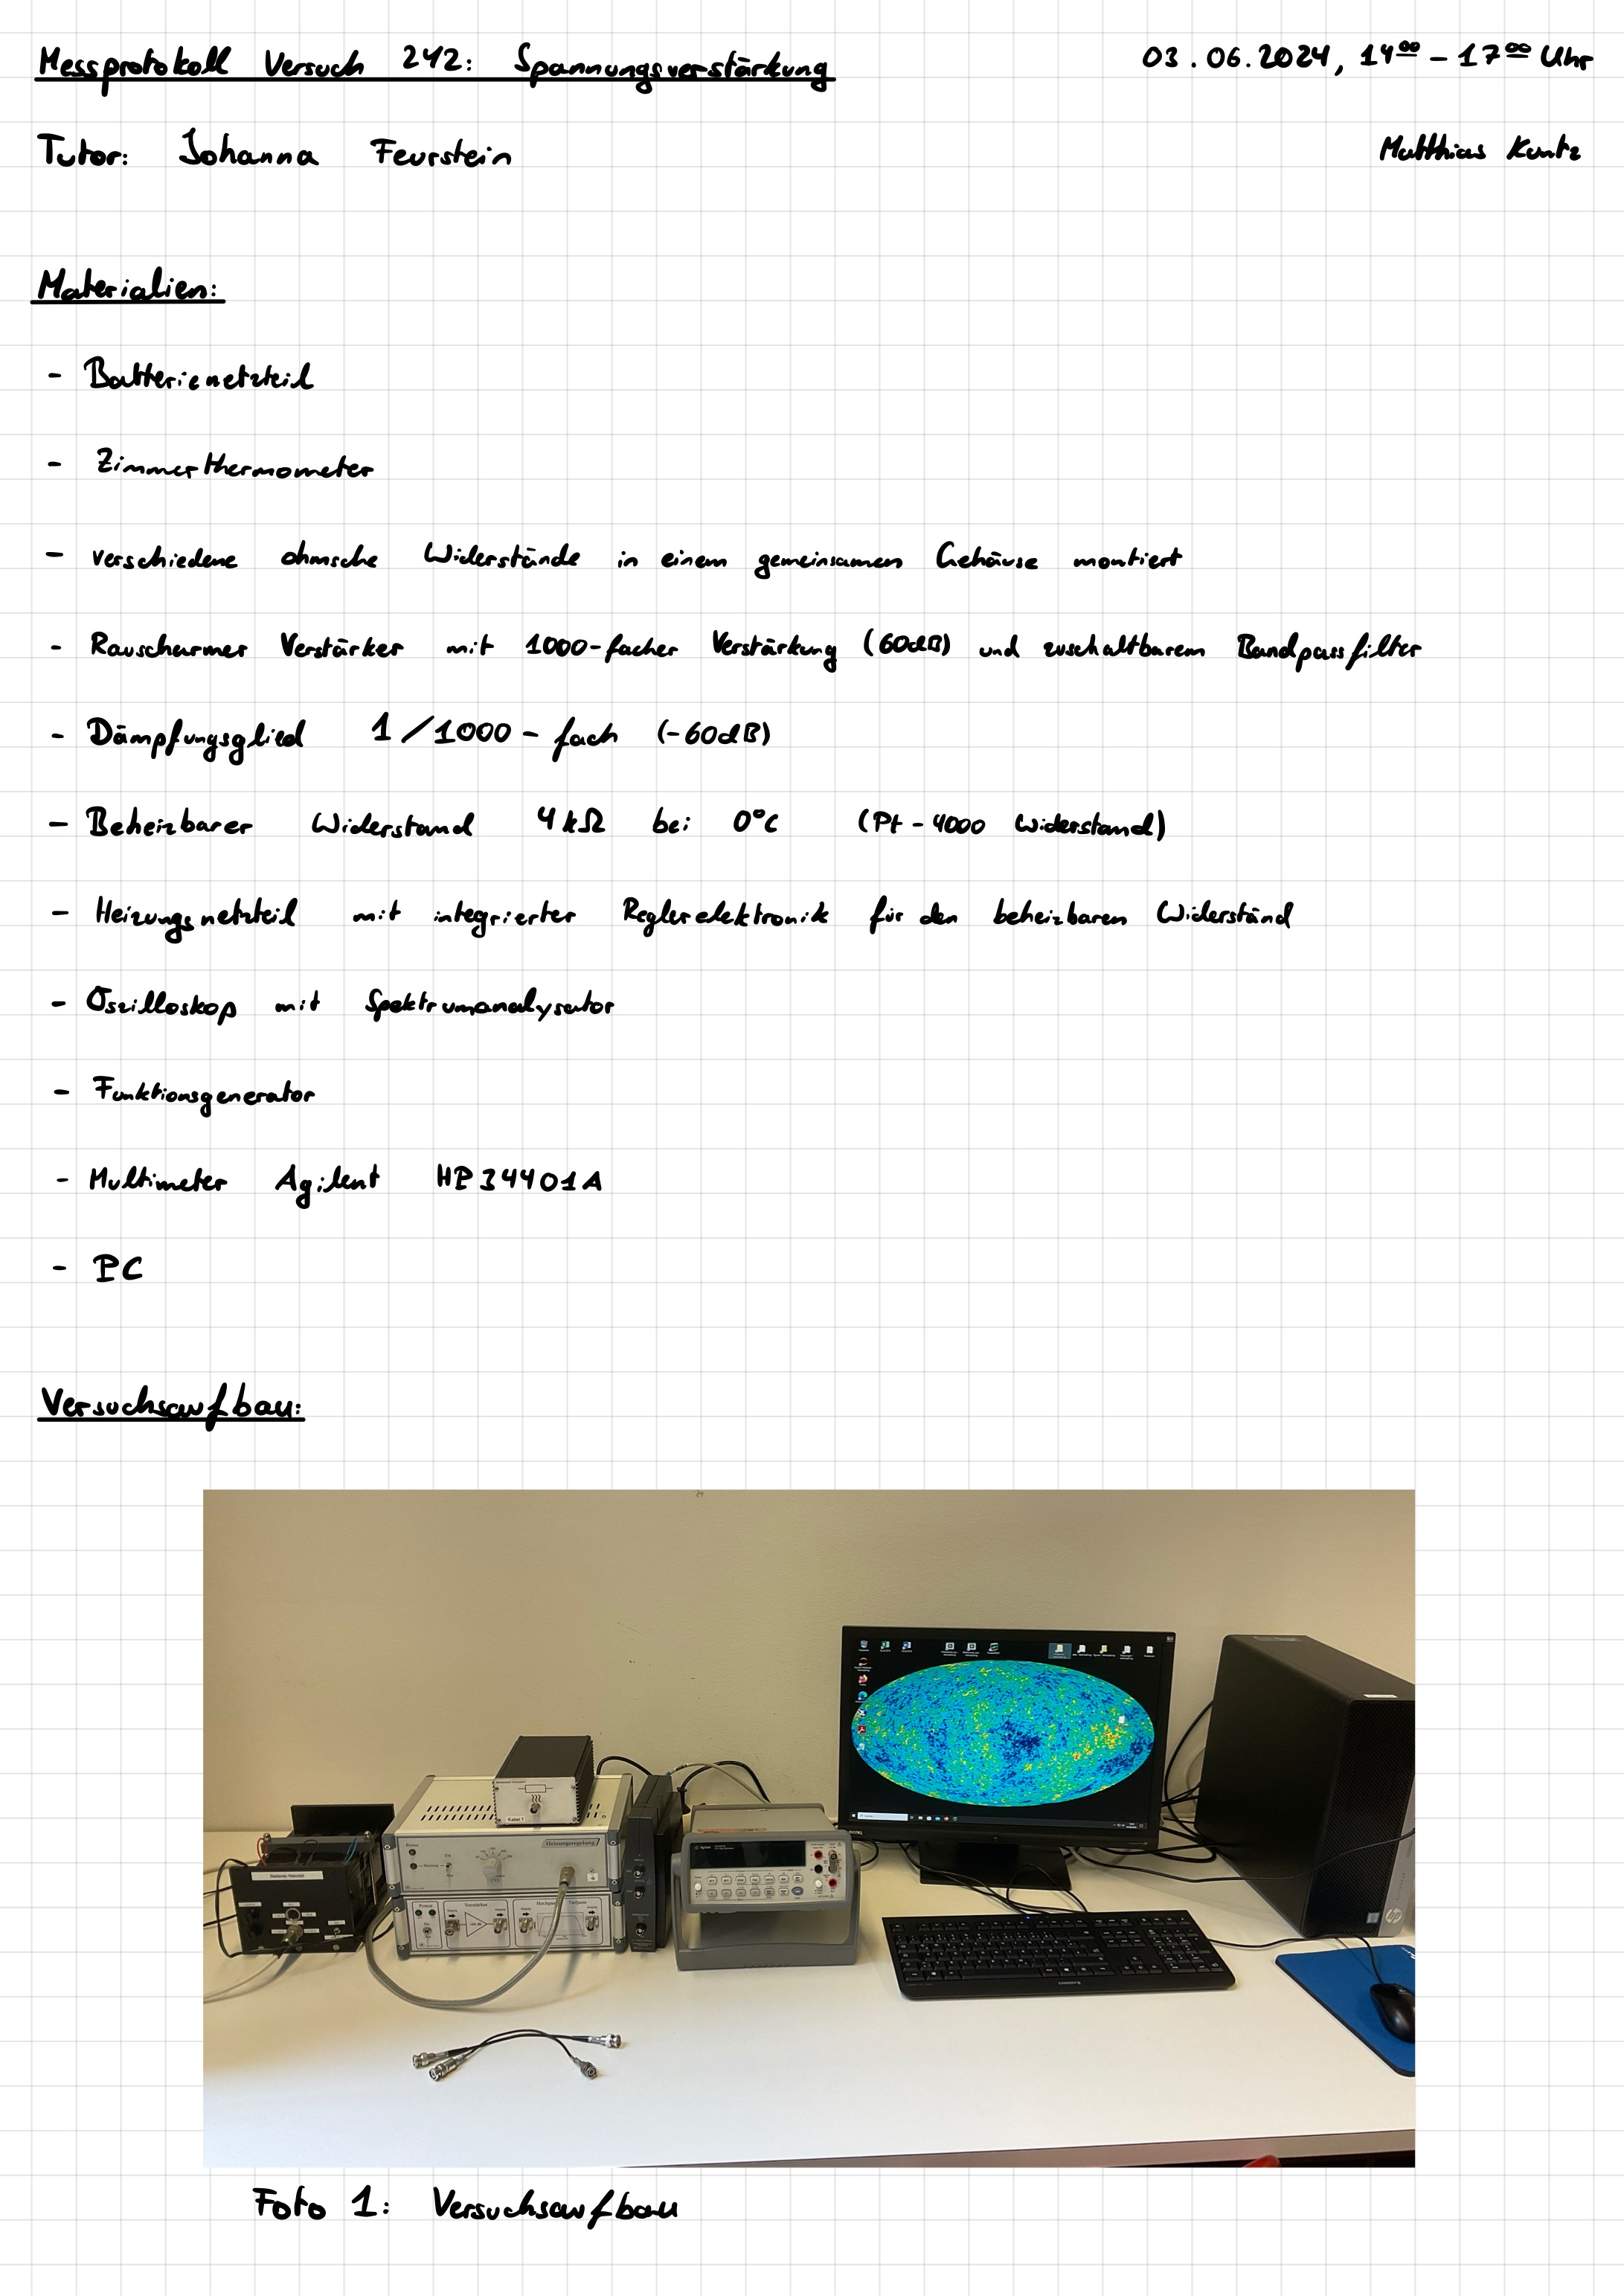
\includegraphics[width=\textwidth]{graphics/mess1.jpg}
\newpage
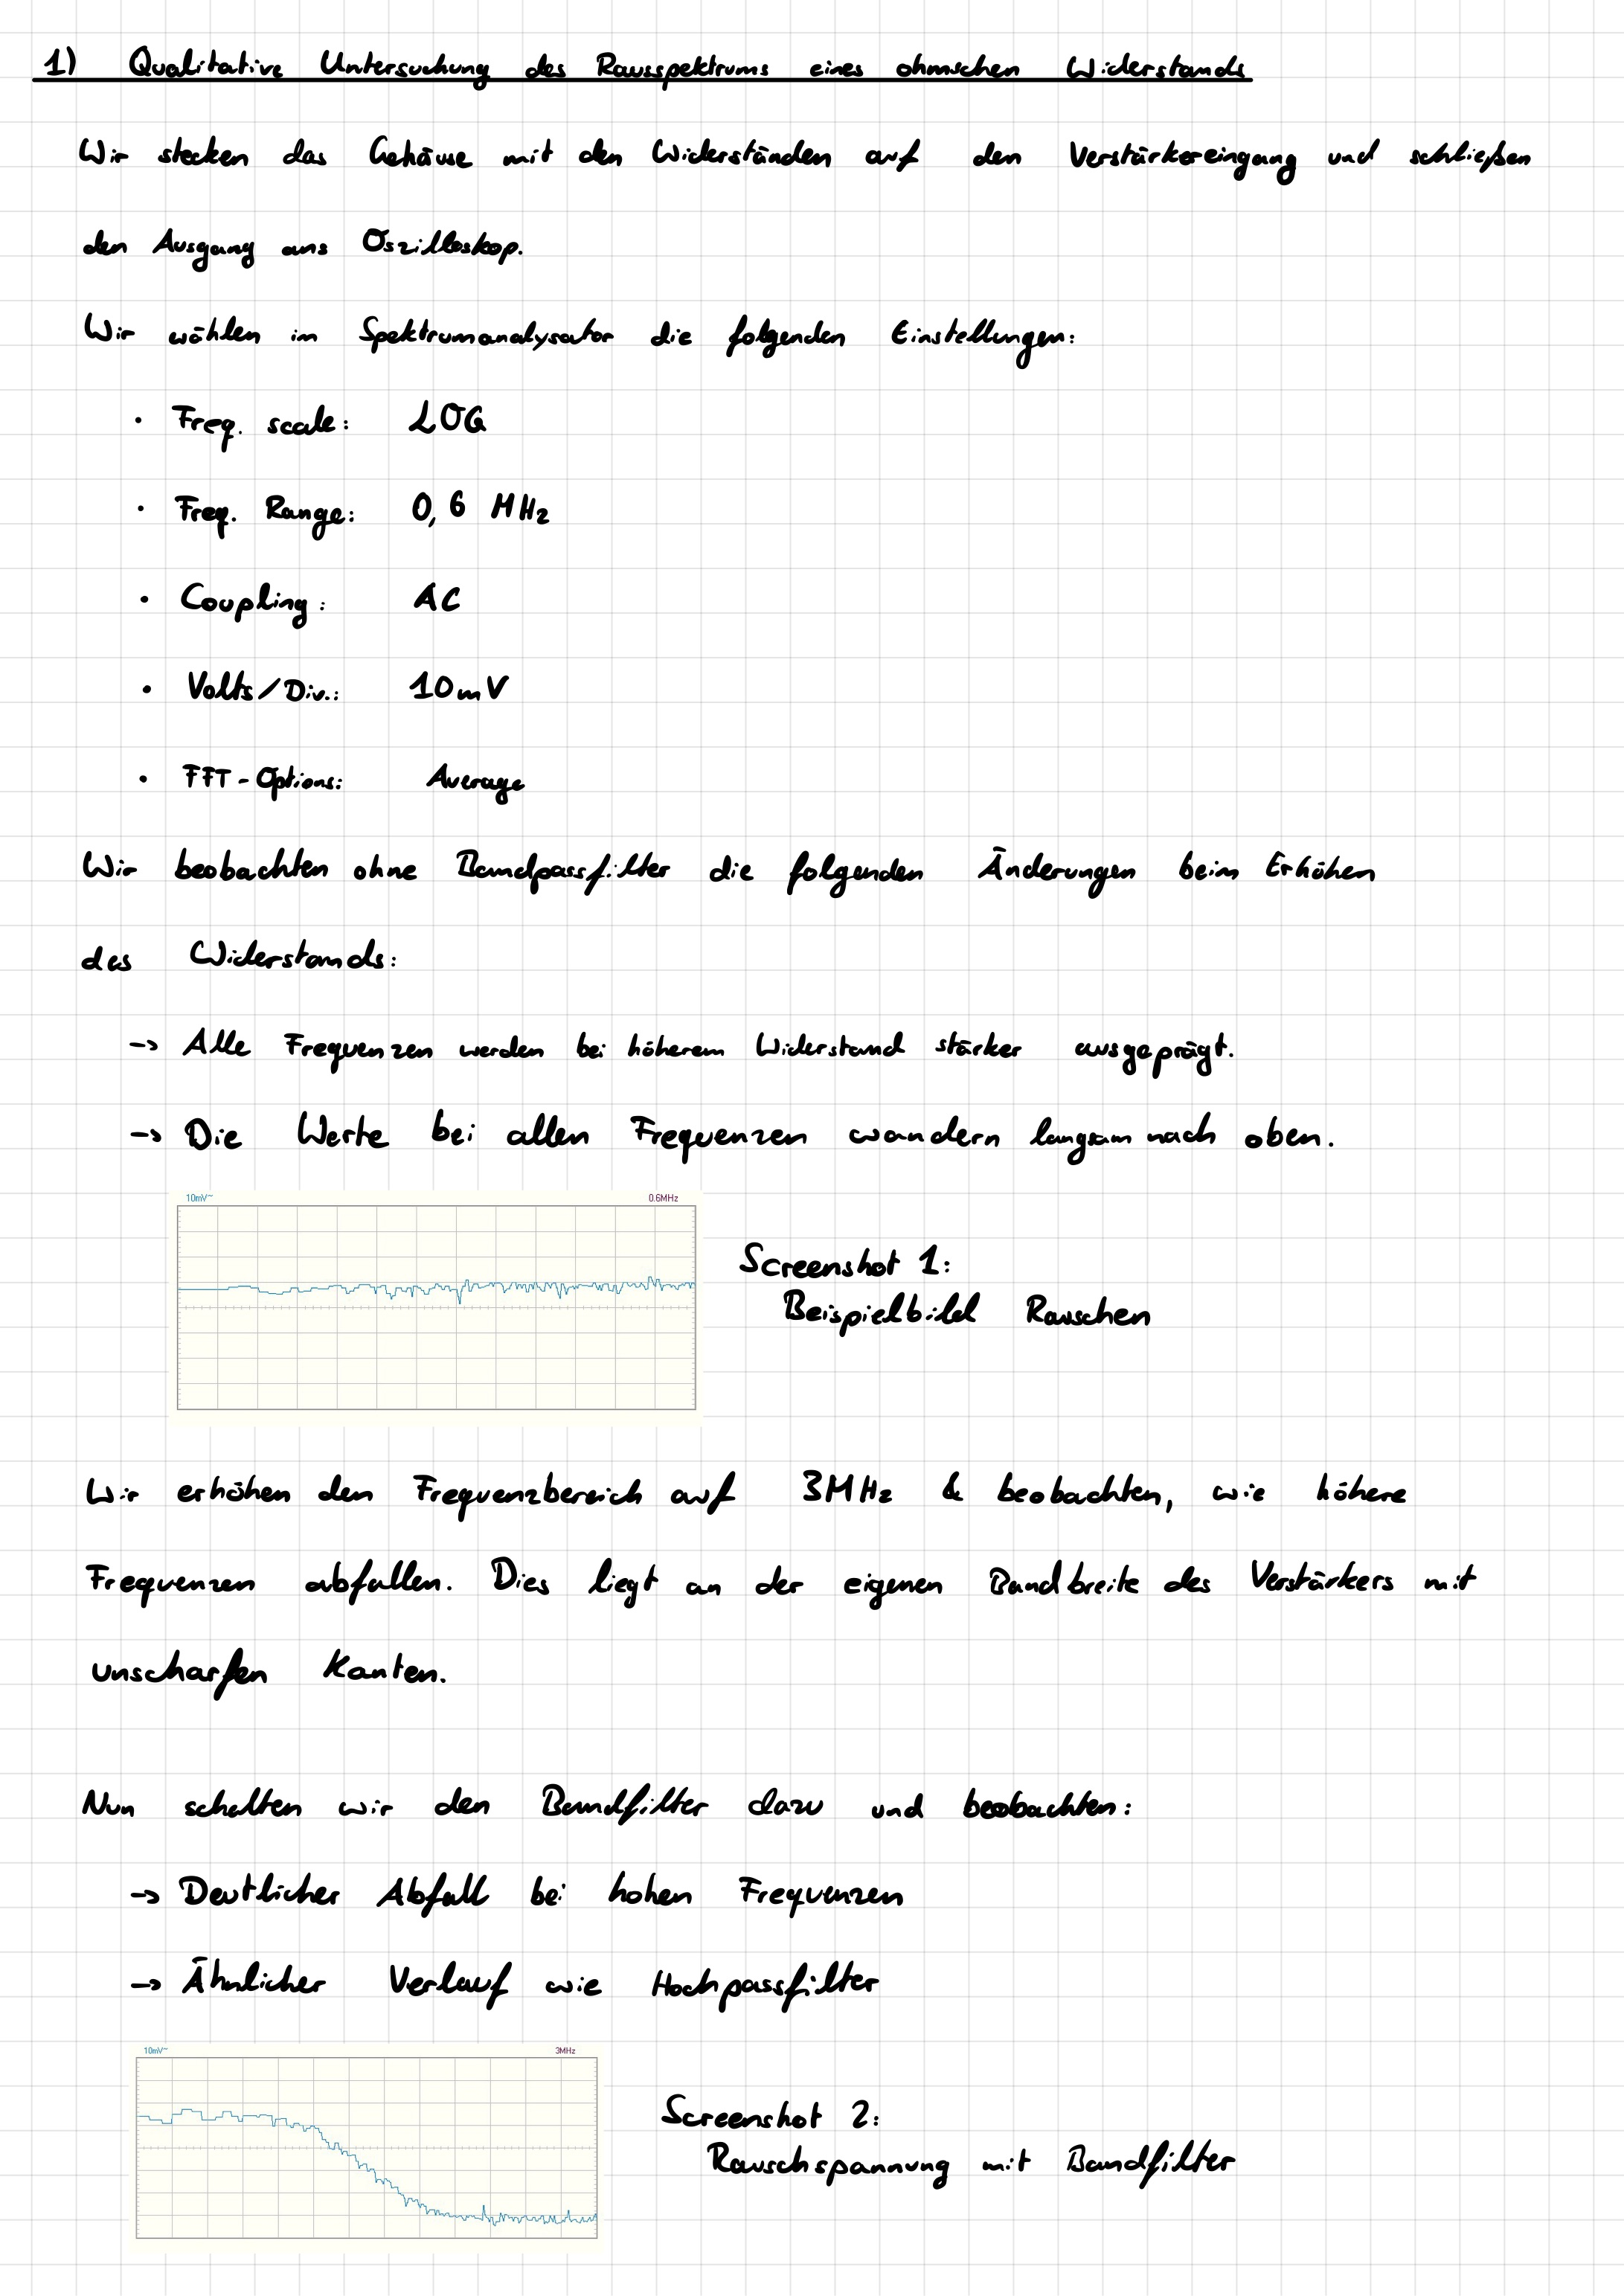
\includegraphics[width=\textwidth]{graphics/mess2.jpg}
\newpage
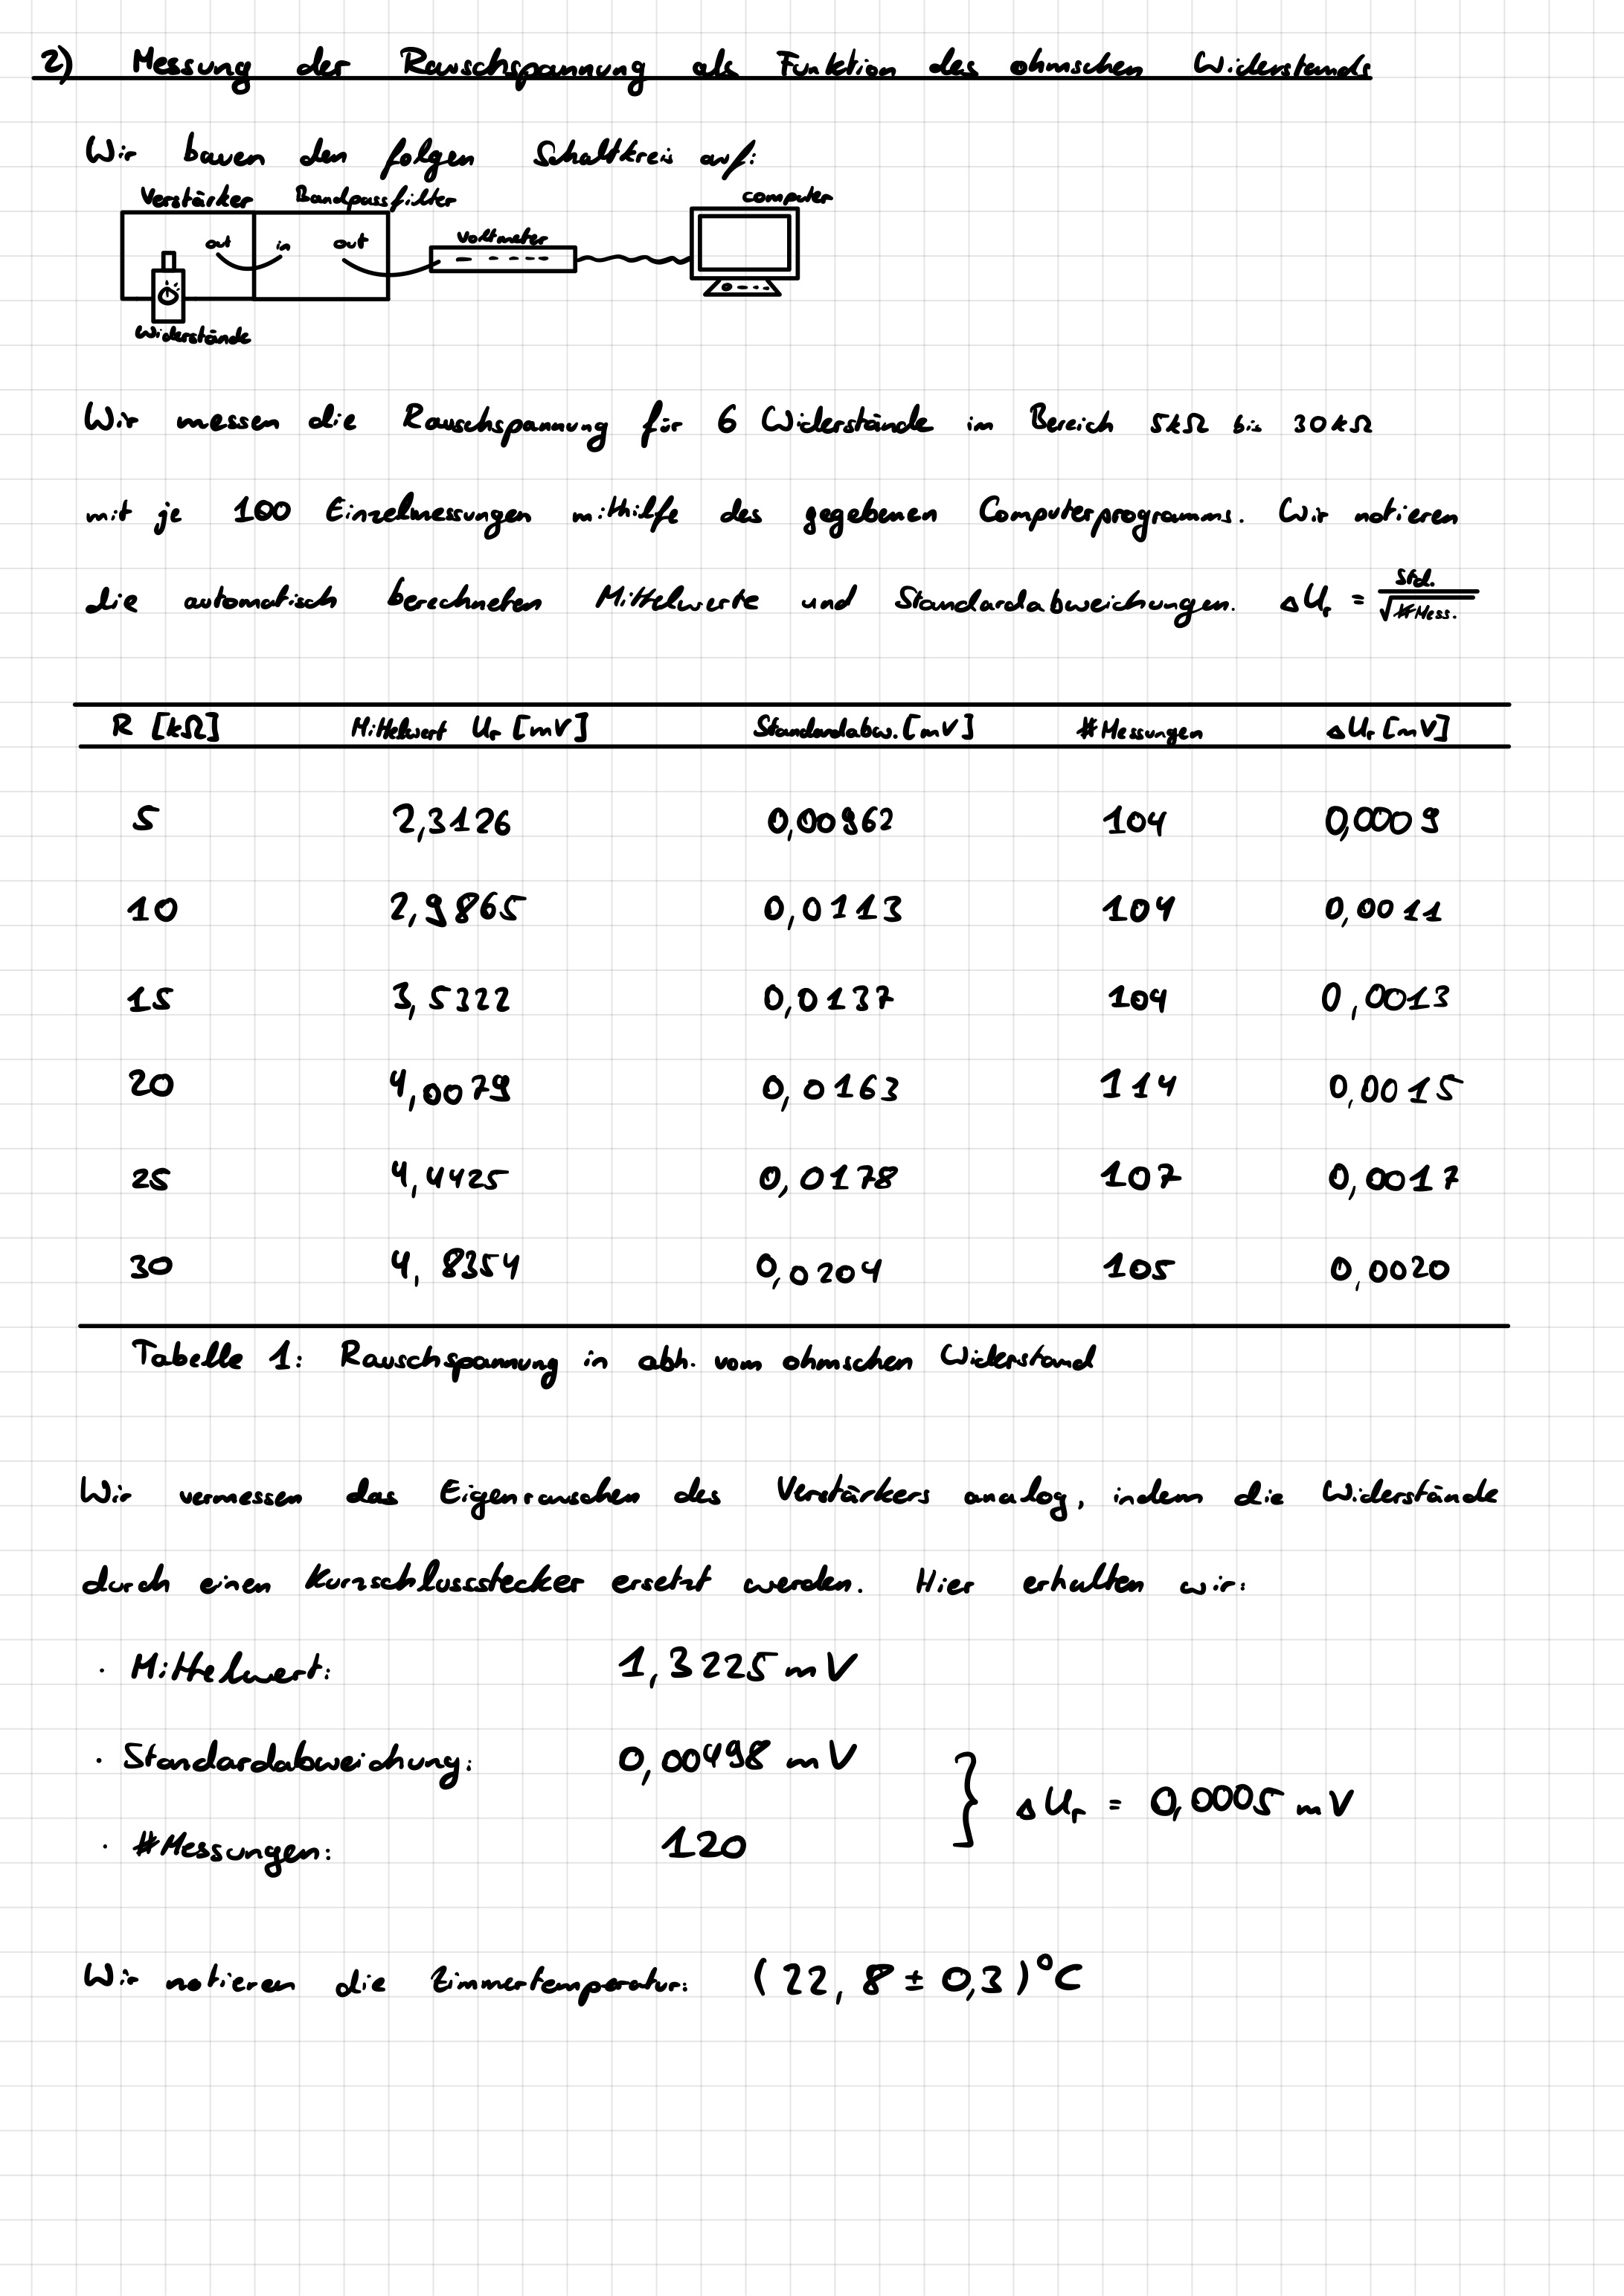
\includegraphics[width=\textwidth]{graphics/mess4.jpg}
\newpage
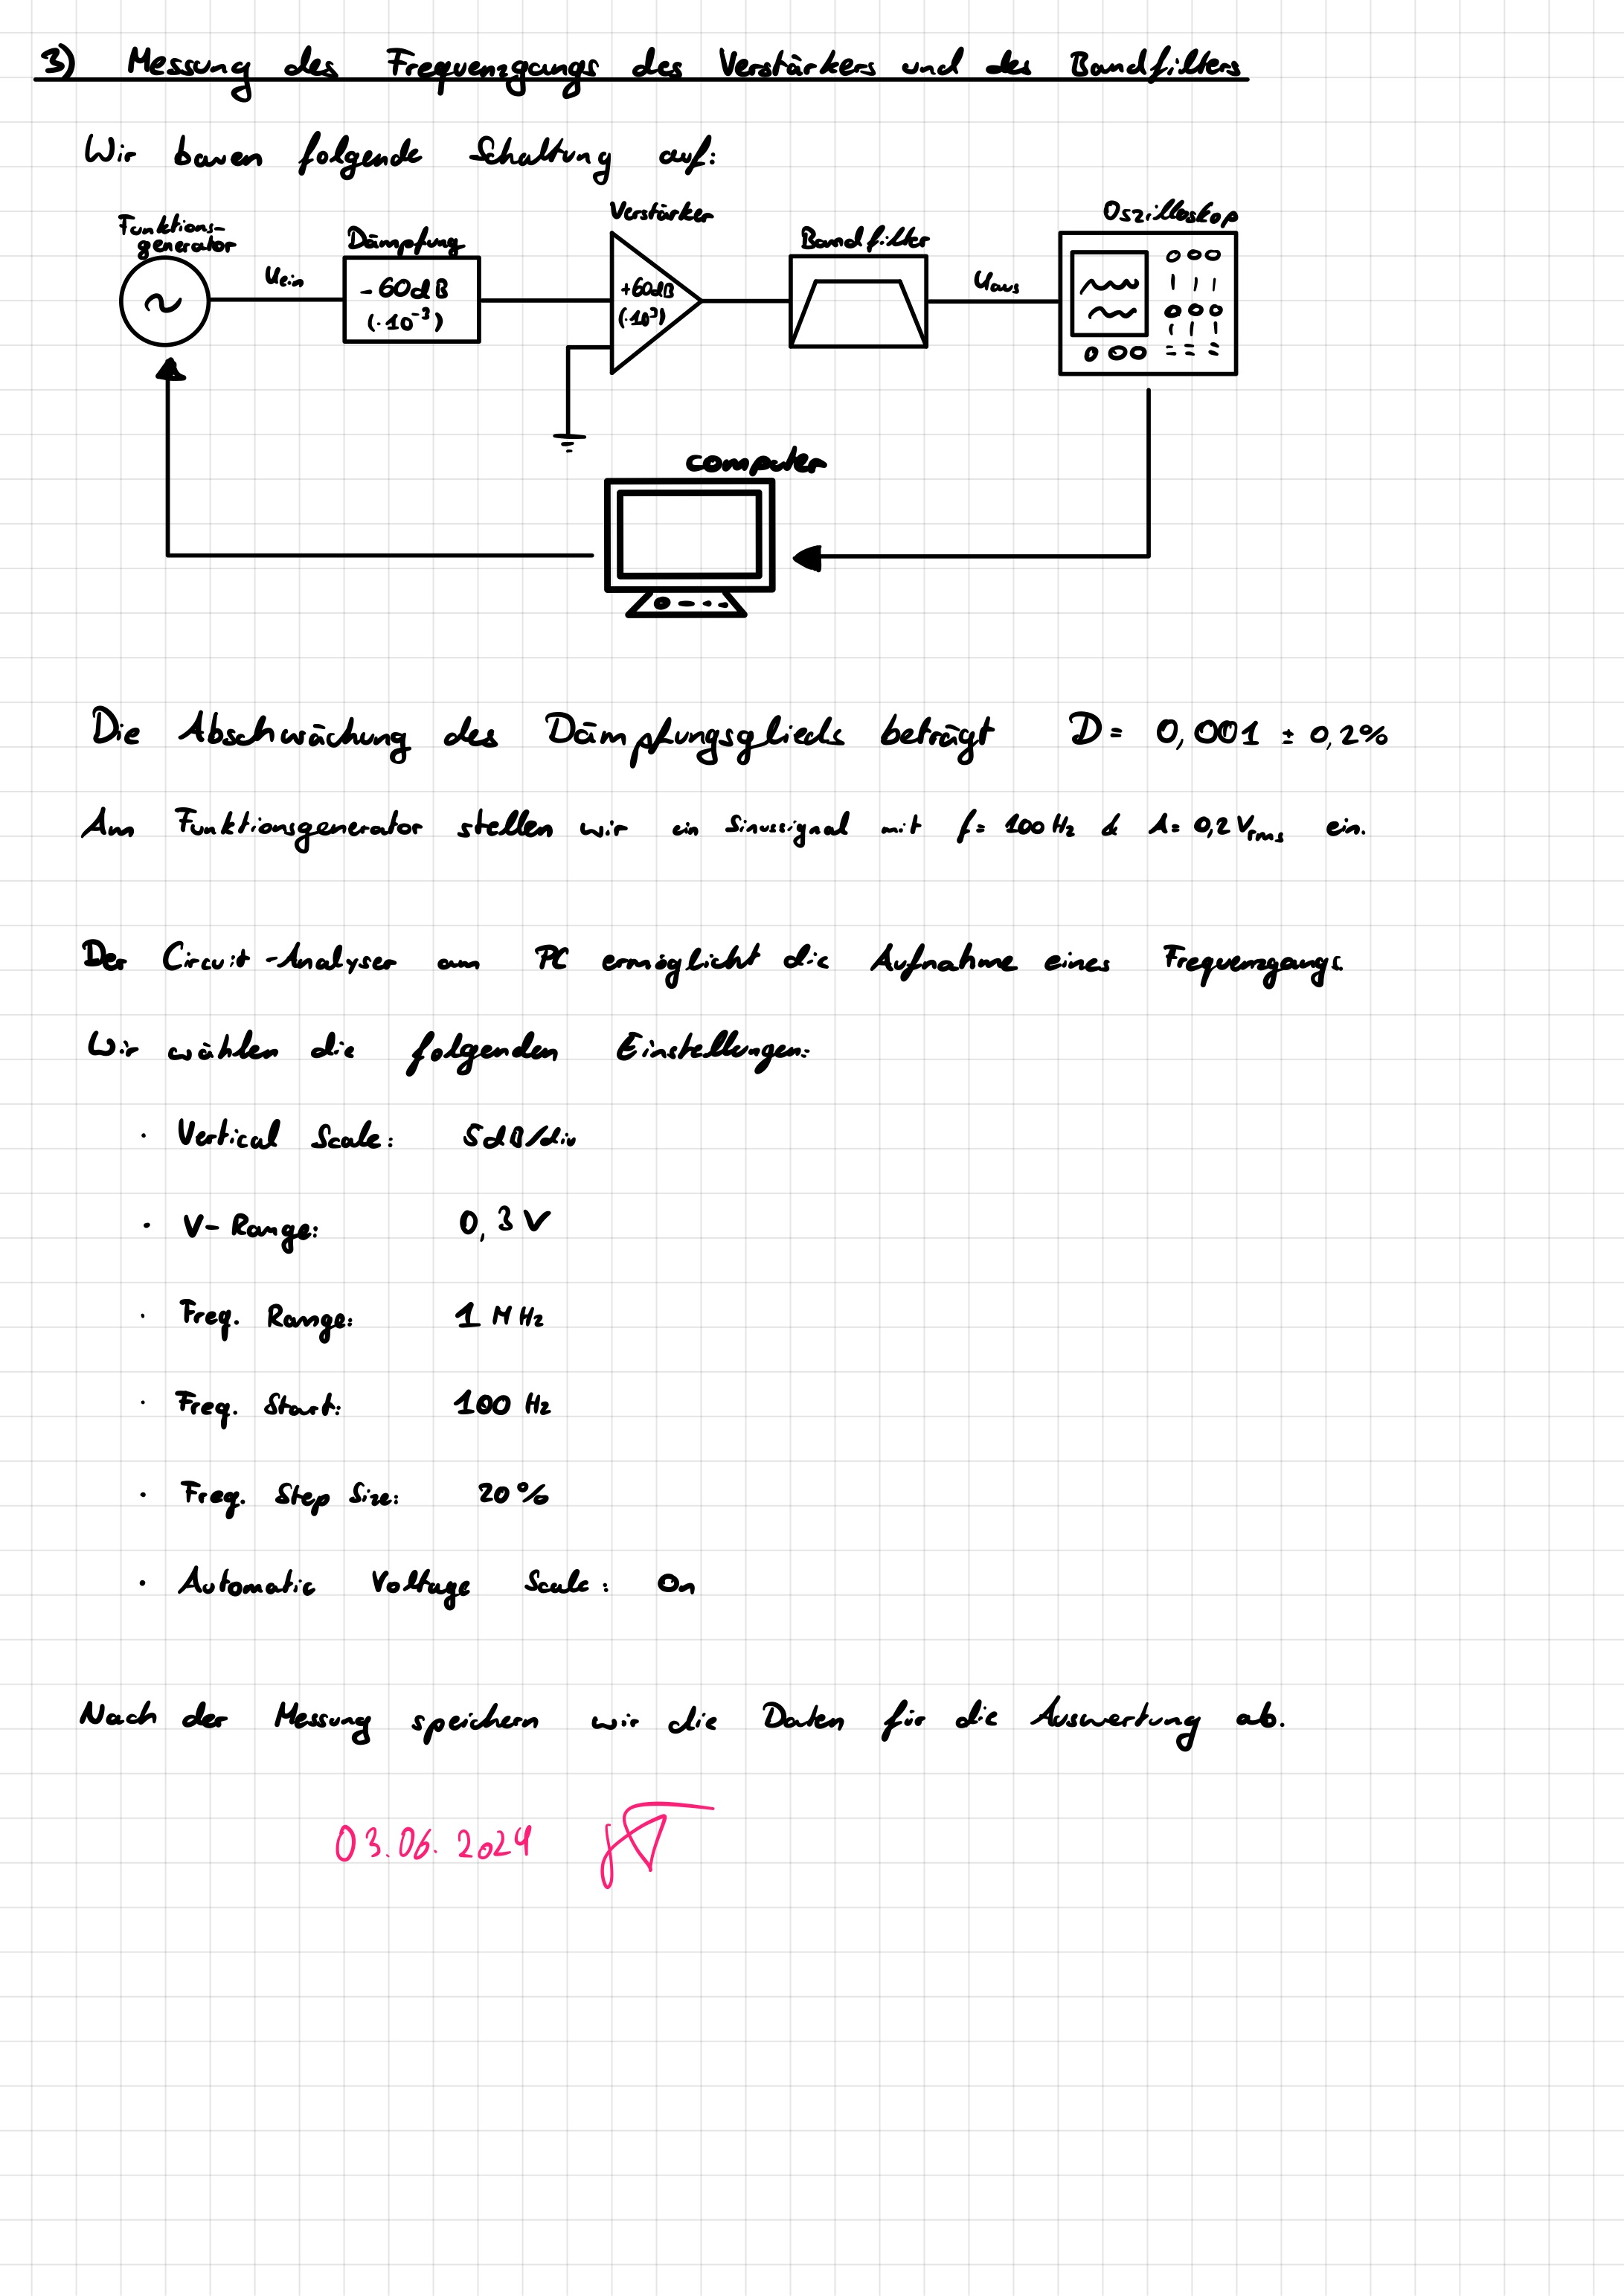
\includegraphics[width=\textwidth]{graphics/mess3.jpg}
\newpage

\addtocounter{table}{1}

\clearpage
\newpage
%-------------------------AUSWERTUNG-------------------------
\section{Auswertung}

In dieser Evaluation werden alle Fehler, sofern keine spezifische Angabe gemacht wird, mithilfe der Gauss'schen Fehlerfortpflanzung berechnet. Dies bedeutet, dass ein Wert $F$, der mit der Formel $f(a_1, ..., a_n)$ berechnet wird, den Fehler $\Delta F$ annimmt:

\begin{equation}
    \Delta F = \sqrt{\sum_n \left( \frac{\partial f}{\partial a_n} \cdot \Delta a_n \right)^2}.
\end{equation}

Des Weiteren erfolgen Signifikanztests von zwei Werten $a$ und $a'$ über die folgende Formel:

\begin{equation}
    \sigma = \frac{|a-a'|}{\sqrt{(\Delta a)^2 + (\Delta a')^2}}.
\end{equation}

Die Auswertung sowie Berechnung erfolgen über das dem Dokument angehängte Python-Programm. Hierbei erfolgen Fits von Funktionen mithilfe der 'curve\_fit'-Funktion des 'SciPy'-Packages und Plots werden mit 'matplotlib' erstellt.

Die Güte eines Fits wird mit der $\chi^2$-Summe bewertet:

\begin{equation}
    \chi^2 = \sum_i^N \left( \frac{\textit{Funktionswert}_i - \textit{Messwert}_i}{\textit{Fehler}_i} \right)^2
\end{equation}

Auch verwendet wird $\chi^2_{red} = \chi^2 / f$, wobei der Freiheitsgrad $f$ die Anzahl der Messwerte minus die Anzahl der Fitparameter ist. Der auf die Freiheitsgrade normierte Wert soll bei einem guten Fit ungefähr 1 sein.


\newpage

\subsection{Auswertung der qualitativen Beobachtungen}

Im ersten Teil des Versuchs beobachteten wir qualitativ, wie unterschiedliche Konfigurationen das Ausgangssignal am Oszilloskop verändern. 

Zunächst erhöhten wir den Widerstand, über dem wir die Rauschspannung messen und stellten fest, dass ein größerer Widerstand eine höhere Rauschspannung erzeugt. Dies entspricht der in der Nyquist-Beziehung gegebenen Relation $\langle U_r^2 \rangle \propto R$ und passt somit zur theoretischen Erwartung. 

Daraufhin konnten wir beobachten, wie ohne zusätzlichen Bandpassfilter die Rauschspannung bei großen Frequenzen aufgrund der eigenen Bandbreite des Widerstands abfällt. Mit zusätzlichem Bandpassfilter konnte ein deutlicherer Abfall bei hohen Frequenzen beobachtet werden, was auf die in der Einleitung beschriebenen schärferen Kanten des Bandpassfilters zurückzuführen ist.

Somit entsprechen alle Beobachtungen den zugrundelegenden Theorien und liefern erwartete Ergebnisse. 



\subsection{Auswertung des Frequenzgangs}

Wir importieren unsere digital gespeicherten Messdaten aus Teil 3 in Python und berechnen den Frequenzgang aus den gemessenen Ausgangsspannungen $U_a$ sowie der gegebenen Eingangspannung $U_a = 0,2$V und Dämpfung $D= 0,001$ gemäß Gleichung \ref{eq:Frequenzgang}. Wir plotten die Punkte, die wir für den Frequenzgang $g(f)$ erhalten, doppellogarithmisch gegen die Frequenz und fitten die folgende Funktion an:

\begin{equation}
    g(f) = \frac{V}{\sqrt{1 + 1 /(f / \Omega_1)^{2n_1}} \sqrt{1 + (f/ \Omega_2)^{2n_2}}}
\end{equation}

Hierbei bezeichnet $V$ die Verstärkung, $\Omega_{1}$ die Grenzfrequenz des Hochpassfilters und $\Omega_2$ die des Tiefpassfilters und $n_{1/2}$ bezeichnen die jeweiligen Fitordnungen. Wir beachten dabei, die sich in Sättigung befindenden Punkte am Anfang und Ende nicht mit zu berücksichtigen.

Der in Abbildung \ref{fig:Frequenzgang+Fit} dargestellte Fit ergibt die folgenden Parameter:

\begin{equation}
    \begin{split}
        V &= 968,2 \pm 2,2 \\
        \Omega_1 &= (1032 \pm 5) \text{Hz} \\
        \Omega_2 &= (45,14 \pm 0,19) \text{kHz} \\
        n_1 &= 4,38 \pm 0,09 \\
        n_2 &= 4,52 \pm 0,08 \\
    \end{split}
\end{equation}

Wir integrieren numerisch das Integral 

\begin{equation}
    B = \int_{0}^{\infty} g(f)^2 df,
\end{equation}

woraus wir den folgenden Wert erhalten:

\begin{equation}
    \bm{B = (4,2189 \cdot 10^{10} \pm 2\%)Hz}
\end{equation}

\phantom{.}

\begin{figure}[!h]
    \centering
    \resizebox{0.9\textwidth}{!}{
    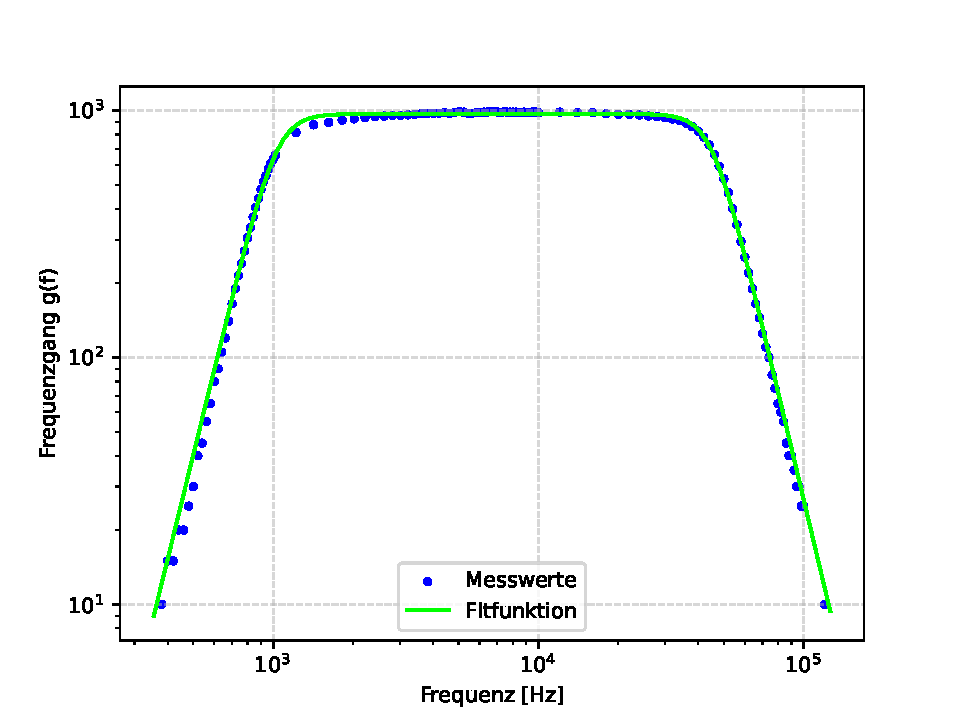
\includegraphics{plots/Frequenzgang.pdf}}
    \caption{Frequenzgang mit Fitfunktion}
    \label{fig:Frequenzgang+Fit}
\end{figure}


\newpage

\subsection{Bestimmung der Boltzmannkonstante}

Wir werten nun Tabelle 1 des Messprotokolls aus. Zunächst berechnen wir die Differenz

\begin{equation}
    \begin{split}
        D &= (U_{r}^2 - U_V^2) \\
        \Rightarrow \Delta D &= \sqrt{(2 U_r \Delta U_V)^2 + (2 U_V \Delta U_r)^2}
    \end{split}
\end{equation}

Diese Werte tragen wir gegen den Widerstand in ein Diagramm und fitten eine lineare Funktion $y = \alpha \cdot x$. Für den in Abbildung \ref{fig:Messdaten+Fit} dargestellten Fit erhalten wir den folgenden Fitparameter und die $\chi^2$-Summe:

\begin{equation}
        \alpha = (7,180 \pm 0,021) \cdot 10^{-10} \frac{\text{V}}{\Omega}
\end{equation}

\begin{equation}
    \begin{split}
        \chi^2_{red} &= 0,2341 \\
        Wsk. &= 95,0\%
    \end{split}
\end{equation}

An dem $\chi^2_{red}$-Wert lässt sich erkennen, dass unsere Fehler etwas zu groß abgeschätzt wurden, insgesamt ist der Fit aber akzeptabel. 

Aus der Steigung bestimmt man nun gemäß Gleichung \ref{eq:Boltzmann} die Boltzmannkonstante. 

\begin{equation}
    \alpha = 4 k_B T B
\end{equation}

Für den Fehler unterscheiden wir zwischen statistischem Fehler aus der Steigung und Temperatur sowie dem systematischen Fehler aus dem numerisch berechneten Wert für $B$. 

\begin{equation}
    \begin{split}
        \Delta k_{stat} &= k_B \sqrt{\left( \frac{\Delta \alpha}{\alpha}\right)^2 + \left( \frac{\Delta T}{T}\right)^2} \\
        \Delta k_{sys} &= k_B \cdot 0,02
    \end{split}
\end{equation}

Somit erhalten wir:

\begin{equation}
    \bm{k_B = (1,438 \pm 0,004 \ \textbf{stat.} \pm 0,03 \ \textbf{sys.}) \cdot 10^{-23}} \frac{\textbf{J}}{\textbf{K}}
\end{equation}

Wir vergleichen diesen Wert mit dem offiziellen NIST CODATA Wert von $k_B = 1,380649 \cdot 10^{-23}$ und erhalten eine Abweichung von $1,96 \sigma$. Dies ist eine insignifikante Abweichung, was unser Ergebnis positiv bestätigt.

\phantom{.}

\begin{figure}[!h]
    \centering
    \resizebox{0.9\textwidth}{!}{
    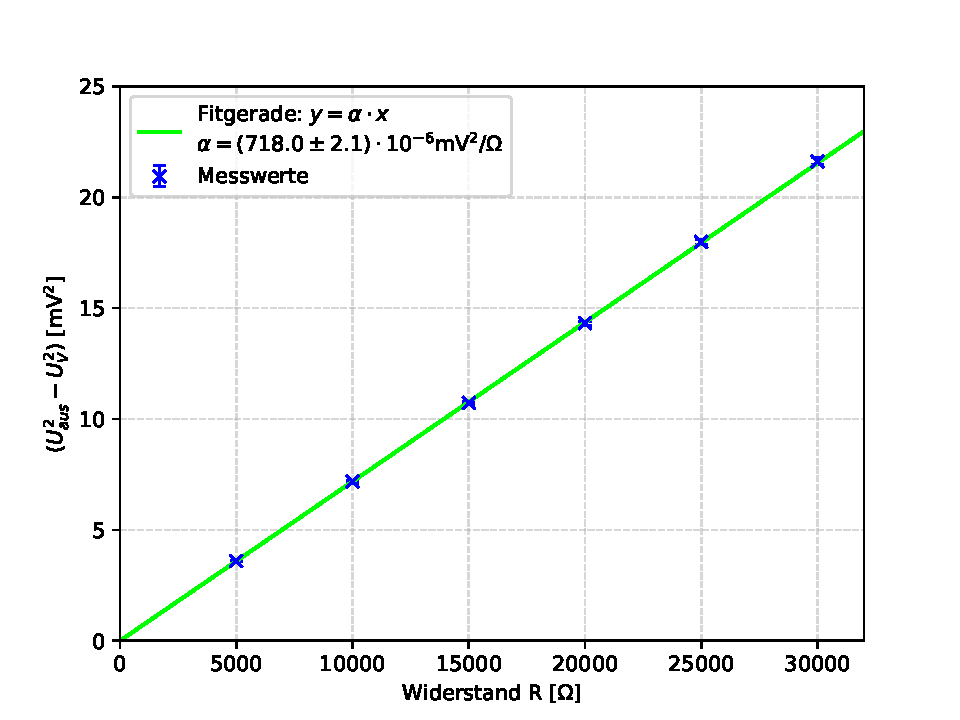
\includegraphics{plots/Steigungsdings.pdf}}
    \caption{Messdaten mit linearem Fit}
    \label{fig:Messdaten+Fit}
\end{figure}

\clearpage
\newpage
%---------------PRÄSENTATION DER ENDERGEBNISSE---------------
\section{Zusammenfassung und Diskussion der Endergebnisse}

In diesem Versuch haben wir mithilfe von thermischem Rauschen in einem elektrischen Leiter die Boltzmannkonstante bestimmt als 

\begin{equation}
    k_B = (1,438 \pm 0,004 \ \text{stat.} \pm 0,03 \ \text{sys.}) \cdot 10^{-23} \frac{\text{J}}{\text{K}}.
\end{equation}

Im Vergleich zum Literaturwert ergab sich eine Abweichung von $1,96 \sigma$. Zusammen mit den zufriedenstellenden qualitativen Beobachtungen kann man also sagen, dass in diesem Versuch durchweg positive Ergebnisse erzielt wurden. Dennoch wollen wir kurz ein paar Aspekte erwähnen.

Potenzielle Fehlerquellen könnten zum einen die Auswertung des Frequenzgangs sowie dessen numerische Integration sein. Bei unserem Plot in Abbildung \ref{fig:Frequenzgang+Fit} ist sehr gut zu erkennen, dass das obere Plateau nicht symmetrisch ist und links etwas schneller abfällt als rechts, was von unserem Fit nicht berücksichtigt wird. Mehr engere Messwerte und ein leicht angepasstes Fitmodell hätten hier ein akkurateres Ergebnis für $B$ erzielt.  

Des Weiteren lässt sich nicht beurteilen, wie akkurat die Methode des Dämpfens und anschließendem Verstärkens ist. Da wir keinerlei exakte Messungen des Dämpfungs- und Verstärkungsgliedes durchgeführt haben und nicht zwangsläufig garantiert ist, dass sich diese beiden exakt aufheben, könnten auch hier leichte Abweichungen entstehen. 

Zusammenfassend lässt sich aber sagen, dass trotz dieser potenziellen Fehlerquellen durchweg Ergebnisse erzielt wurden, die mit der Theorie übereinstimmen und der Versuch somit aussagekräftige und positive Resultate ergab.  




 
\newpage
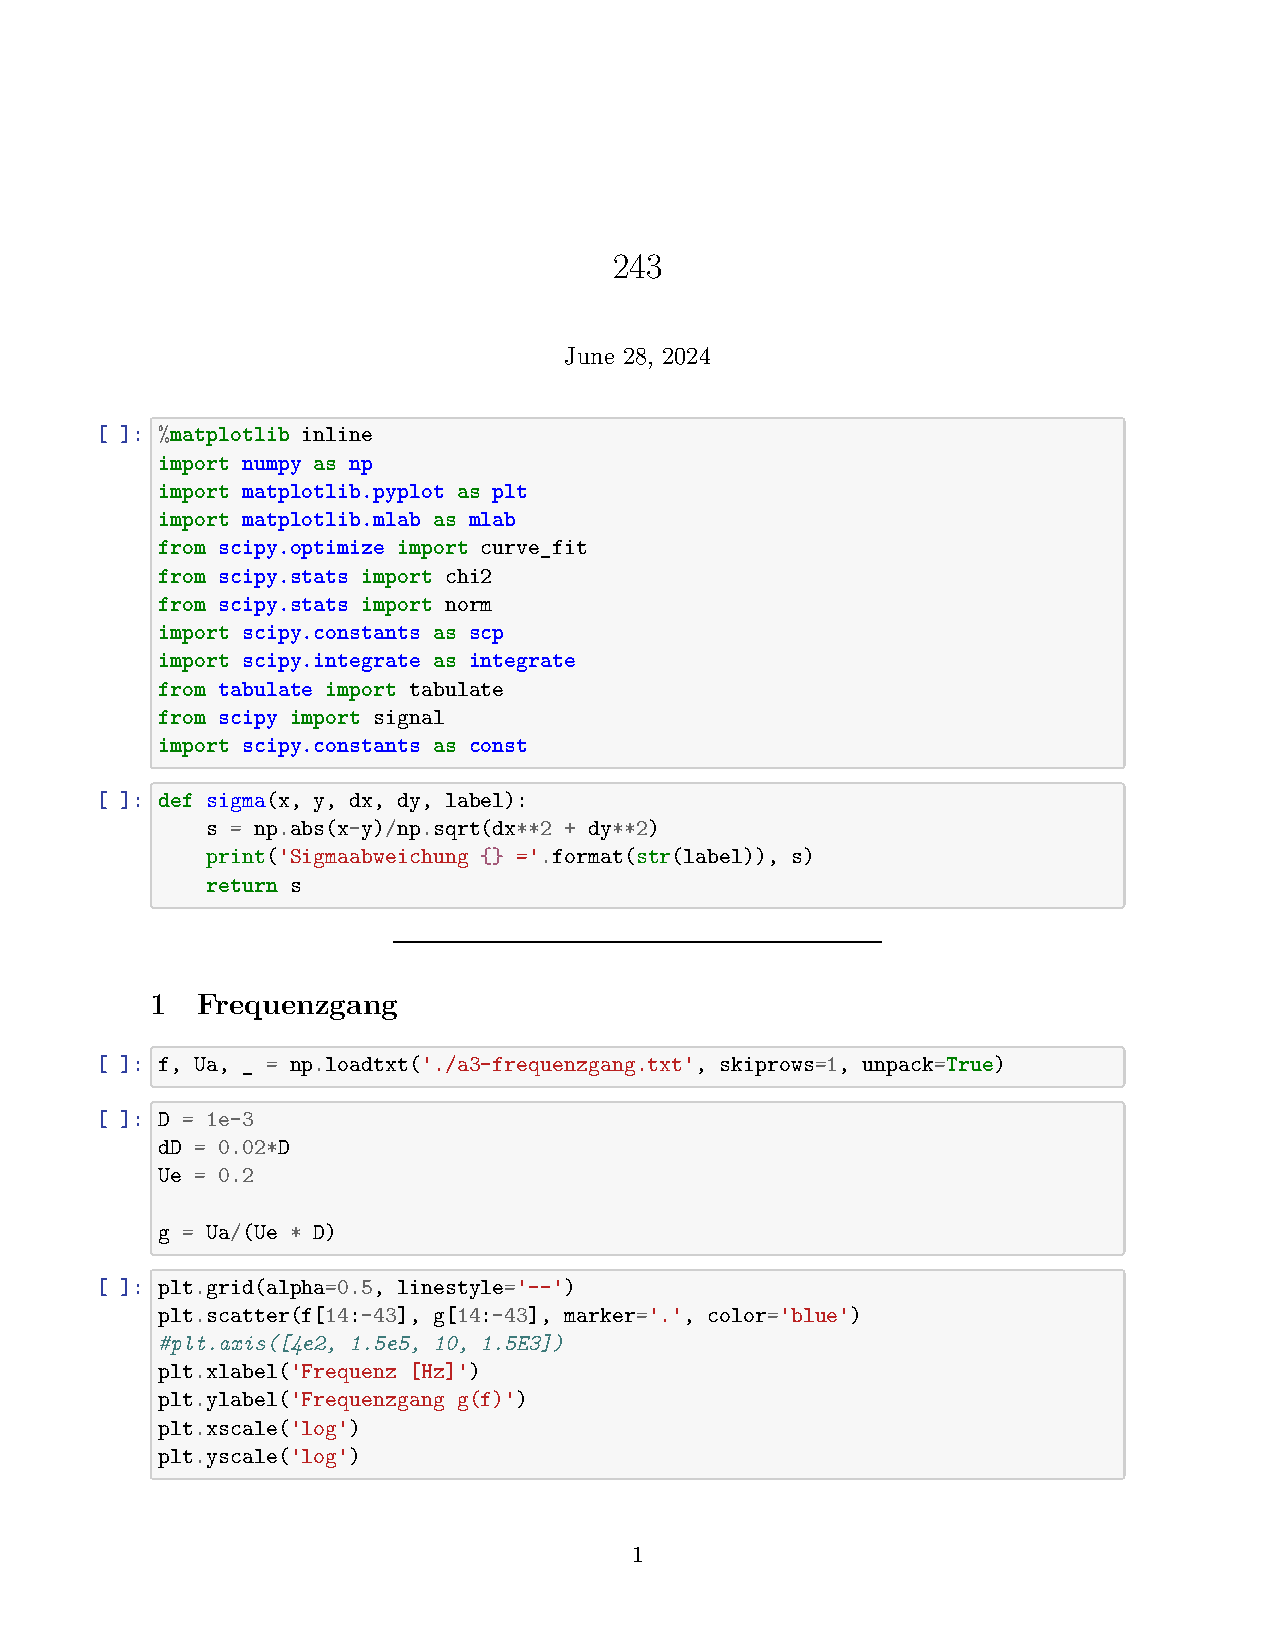
\includepdf[pagecommand=\invisiblesection{Python-Code},scale=0.8,pages=1]{243.pdf}
\includepdf[pagecommand={},scale=0.8,pages=2-last]{243.pdf}

\end{document}

